

Fuzz testing is a popular technique for automatic software vulnerability detection 
 \cite{Miller:Fuzz, 5010257, sutton2007fuzzing}.
 However, it suffers from the low efficiency bottleneck when being applied to real-world software 
 \cite{neystadt2008automated, godefroid2008automating, ganesh2009taint, cadar2011symbolic, rawat2017vuzzer, stephens2016driller},
  which often has complex input formats, e.g., Portable Document Format (PDF).
  Most of the test cases generated by fuzz testing will be discarded on the shallow surface of such software.
  In order to improve the performance of traditional fuzz testing, 
  coverage-based fuzz testing collects all the test cases that contribute to the coverage into a seed file queue,
  and generates the test input from the seed files in each cycle of mutation using genetic methods
  \cite{rawat2017vuzzer, online:afl, stephens2016driller}.
  Although coverage-based testing is able to reach more paths than traditional fuzz testing, 
  due to the usage of random mutation,
  it is nevertheless incapable of triggering bugs that are deeply nested in complex code areas.


Another technique to improve the efficiency of fuzz testing is symbolic execution assisted hybrid testing \cite{yeh2015craxfuzz, majumdar2007hybrid, pak2012hybrid}.
 In such hybrid testing, symbolic execution is exploited to cover the corner cases that are difficult for classical fuzzers to cover by solving the corresponding path conditions.
 Meanwhile, symbolic execution can also benefit from the seed files in the queue from fuzzer 
 to quickly reach more wider code areas. 
 Driller, which is built on top of Angr symbolic execution engine \cite{Shoshitaishvili_firmalice-automatic} and AFL fuzzing engine \cite{online:afl}, 
 has attempted to leverage symbolic execution to solve the branches guarded 
 by complex path conditions to avoid the saturation of fuzzer \cite{stephens2016driller}. 
 And its performance in the Cyber Grand Challenge (CGC) from DARPA \cite{online:CGC} demonstrates the potential of this hybrid testing approach.


In hybrid testing, the performance gain from symbolic execution is still limited 
 by some certain program structures(e.g., symbolic pointers and loops) \cite{schwartz2010all, Boonstoppel:RAP, cadar2011symbolic, baldoni2016survey}. 
 Such structures will quickly generate many states that cannot trigger new behaviors,
 but raise the intrinsic \textit{path explosion} problem.
 Moreover, by leveraging symbolic execution, 
 the seed queue (including the initial seeds) of the fuzzer will quickly reach a large number for modern software. 
 So when given the testing time budget, the seed queue should be rearranged to make sure 
 that test case with greater probability of triggering new paths will be scheduled with high priority.


 In this paper, we propose two advanced techniques to improve the efficiency of symbolic execution assisted hybrid testing.

 On one hand, symbolic pointers are lazily concretized to avoid generating too many states but cover more branches; and an optimization based on the loop bucket mechanism of AFL \cite{online:afl} is introduced to avoid getting stuck in symbolic loops.
 
 On the other hand, to address the large size of seed queue, 
 we propose a distance based seed selection method for fuzz testing to improve the coverage when testing time is limited. 
 Each test case in the seed file queue is equipped with an weight value.
 This value is obtained from the execution runtime information,
 which includes both path coverage and memory coverage.
 Our method prioritizes the seed queue according to this weight value and 
 then selects the seed file with the greatest weight value for next mutation cycle.



Figure~\ref{Framework} shows the high-level overview of our prototype.

 Our main contributions consist of two main components, namely \emph{Symbolic Path Finder (SPF)} and \emph{Seacher}. 
 The \emph{SPF} component is leveraged to help the fuzzer to dive into deeper code areas 
 that are guarded by complex path constraints. 
 Technique to handle the \textit{path explosion} problem 
 raised by symbolic pointers and loops is implemented inside of \emph{SPF}. 
 The \emph{Searcher} is designed to select the most promising seed file 
 from the seed queue based on the distance measurement. 
 By doing this, the fuzzer will touch more virgin code areas as soon as possible in a time budget. 

 Least but not last,  we have implemented the proposed techniques in a prototype tool,
 and performed a comprehensive experimental evaluations on three different benchmarks. The benchmarks consist of a demo program which contains 9 different difficult level bugs, recently released LAVA benchmark \cite{dolan2016lava}, and a set of real world UNIX programs. 
 The results show that our prototype can increase the coverage by 34.3\% and trigger more bugs than the state-of-the-art vulnerability discovery tools.


\begin{figure}
\begin{center}
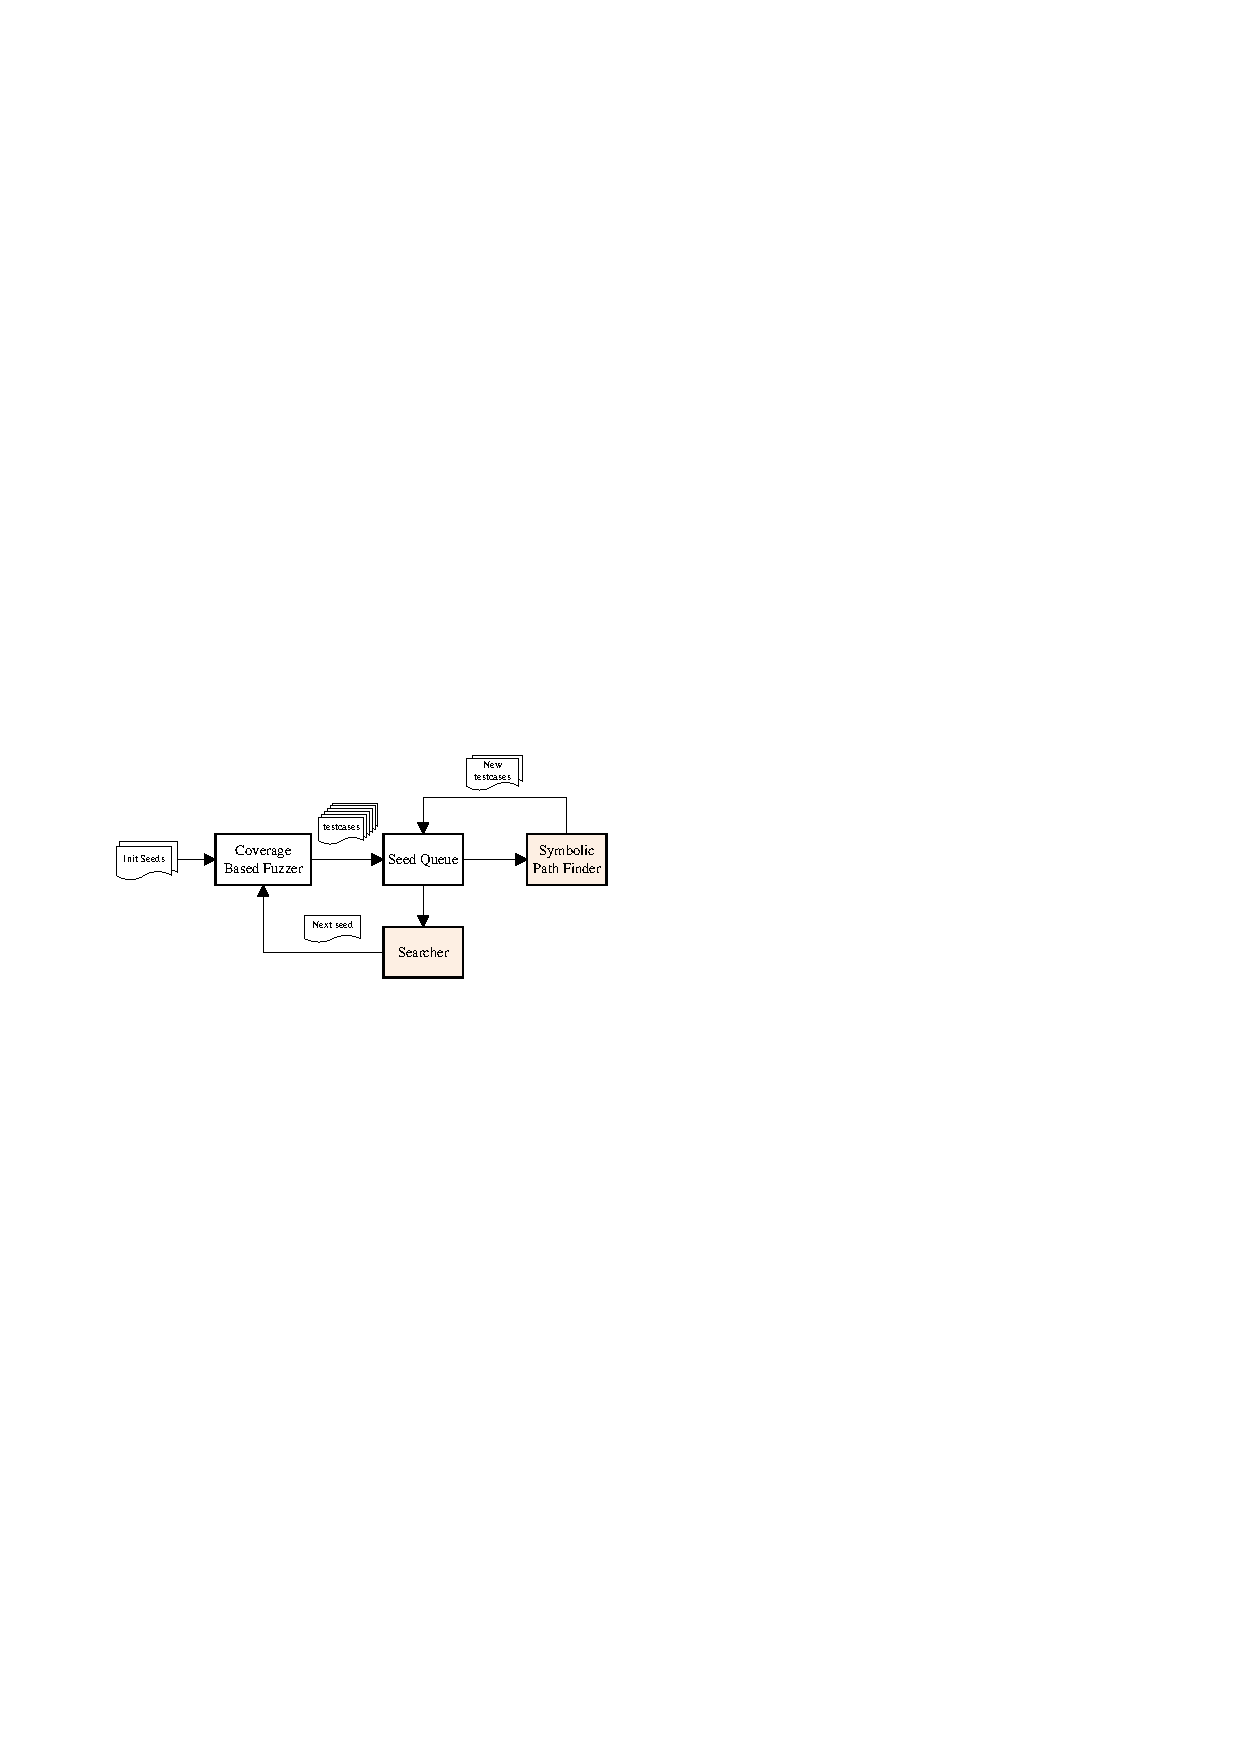
\includegraphics[width=0.7\textwidth]{figures/framework.pdf} 
\caption{High Level Framework.}\label{Framework}
\end{center}
\end{figure}


In summary, this paper makes the following contributions.
\begin{itemize}
\item We introduce a technique to avoid forking more states by postponing the concretization of symbolic pointer to the moment when branch condition depends on such pointer.  
 We also present an optimization namely \emph{symbolic loop bucket} to ease the \textit{path explosion} problem by limiting the looping times to a serial of fixed buckets.

\item A \emph{distance based seed selection} method is proposed to select the most promising seed 
 in the queue according to the runtime information (i.e., path coverage and memory coverage) to improve path discovery when testing time is limited. 

\item We have implemented a prototype based on our method, 
 and the evaluation results on several benchmarks demonstrate the capability of our method for different viewpoints.
\end{itemize}


The rest of this paper is organized as follows. 
 Section~\ref{sec:preliminaries} describes the basic conception of symbolic execution and hybrid testing. 
 Section~\ref{sec:ease PE} presents the technique details of how we deal with \textit{path explosion} raised from symbolic pointers and loops. The distance based seed selection method is discussed in Section~\ref{sec:seed selection}. Section~\ref{sec:evaluate} describes the implementation of our prototype and the evaluation results. Section~\ref{sec:discussion} discusses the limitations of our work and possible counter measures. Section~\ref{sec:related} reviews the related work, and Section~\ref{sec:conclusion} concludes this paper.
